% ARCTO: A Profile-Driven Compression Library for AMD GPUs
% Target venue: SBAC-PAD 2026
% Working draft.
\documentclass[conference]{IEEEtran}

\usepackage[T1]{fontenc}
\usepackage{graphicx}
\usepackage{booktabs}
\usepackage{amsmath}
\usepackage{amssymb}
\usepackage{hyperref}
\usepackage{xcolor}
\usepackage{listings}
\usepackage{algorithm}
\usepackage{algpseudocode}

% Useful macros
\newcommand{\arcto}{\textsc{ARCTO}}
\newcommand{\nvcomp}{\textsc{nvCOMP}}
\newcommand{\hipcomp}{\textsc{hipCOMP}}
\newcommand{\TODO}[1]{\textcolor{red}{\textbf{[TODO: #1]}}}

\title{ARCTO: A Profile-Driven Compression Library\\
       for AMD GPUs}

\author{
  \IEEEauthorblockN{Cristiano A. K\"unas, \TODO{co-authors}}\\
  \IEEEauthorblockA{
    Universidade Federal do Rio Grande do Sul (UFRGS), PCAD Lab\\
    Porto Alegre, Brazil\\
    \texttt{cakunas@inf.ufrgs.br}
  }
}

\begin{document}
\maketitle

\begin{abstract}
\TODO{Abstract: write last. ~200 words. Key claims:
(1) AMD has no production-grade GPU compression library;
(2) hipify port from nvCOMP gives functional baseline but is far from
optimal; (3) ARCTO closes this gap with two profile-driven
optimizations -- wave-saturation chunk-size formula
(kernel-side, up to 2.87x kernel speedup on MI300X) and adaptive
tiled aggregation (transfer-side, up to 2.26x end-to-end speedup on
MI300X for 16 GB workloads, vs single-shot pinned which is shown to
be negative in honest accounting). The methodology generalizes to
RDNA and CDNA across four generations, and is validated on the TTI
seismic workload that motivates the work.}
\end{abstract}

\section{Introduction}
\label{sec:introduction}

Modern scientific computing faces an increasingly critical
challenge: the volume of data generated by simulations is growing
faster than the ability to move it efficiently. High-performance
computing applications such as seismic forward modelling, climate
simulation, and molecular dynamics produce datasets ranging from
gigabytes to petabytes, making data movement the dominant
bottleneck in many workflows~\cite{jin2024concealing,lee2002migration}.
GPU-accelerated compression has emerged as an attractive solution,
leveraging the parallel architecture of graphics processors to
achieve throughputs that can exceed storage system
bandwidths~\cite{nvcomp,knorr2021ndzip}.

The high-performance computing landscape, however, has become
increasingly heterogeneous. AMD GPUs now power three of the top ten
systems on the TOP500 list, including the two highest-ranked
exascale systems (El Capitan and Frontier)~\cite{top500nov2025}.
Despite AMD's growing presence in HPC, the availability of optimized
GPU compression tools has not kept pace with the hardware. The
NVIDIA ecosystem benefits from \nvcomp~\cite{nvcomp}, a
vendor-supported, production-ready library available since 2020
that offers architecture-tuned implementations of LZ4, Snappy,
Cascaded, GDeflate, ANS, BitComp, and (since release 5.x) ZFP. In
contrast, the HIP/ROCm ecosystem relies on community-driven efforts
such as \hipcomp{}, which appeared in 2022 and remains experimental,
with limited algorithm coverage, direct-port optimization, and
sparse documentation. This asymmetry creates a tooling vacuum for
the growing number of HPC systems built on AMD GPUs.

A functional hipify-based port of \nvcomp{} establishes an
AMD-compatible baseline~\cite{anon_iccsa2026,kunas2025compressao},
but the resulting implementation is far from optimal: it inherits
launch geometries and host-to-device staging strategies that were
tuned for NVIDIA hardware, leaving substantial throughput on the
table. Recent work on seismic reverse-time migration pipelines
also showed that, even with a correctly ported library, the I/O
subsystem dominates end-to-end time~\cite{kunas2024carla,
boito2017seismic}, which makes the host-to-device staging on the
input path a high-leverage optimization target. Two observations
from a systematic cross-architecture characterization campaign on
AMD's CDNA and RDNA lineups motivate the present work. First, at the kernel level, the default chunk size of 64~KB
inherited from \nvcomp{} leaves the larger AMD parts (notably the
MI300X) wave-count-starved: the number of chunks dispatched is one
to two orders of magnitude smaller than the GPU's wave slot
capacity, and the SIMT pipelines run nearly idle. Second, at the
transfer level, the dominant cost in end-to-end execution is the
host-to-device staging of the input batch, which a naive
per-chunk \texttt{hipMemcpyAsync} from pageable storage caps at
roughly 6~GB/s on PCIe Gen4 -- a fifth of the bus theoretical
peak.

This paper presents \arcto, a profile-driven GPU compression
library for AMD that closes both gaps with two complementary
contributions:

\begin{itemize}
\item A \textbf{wave-saturation chunk-size formula}, derived from
hardware performance counter analysis, that picks the chunk size
which keeps every wave slot busy and unlocks 1.4--2.9x additional
throughput on the compress kernels with no code change other than
a single launch-time parameter.

\item An \textbf{adaptive tiled aggregation API}, derived from a
cost model fitted to the characterization data, that replaces the
single-shot coalesced pinned-host staging used by the published
ICCSA baseline. We show that the single-shot path, when measured
honestly with full lifecycle accounting (\texttt{hipHostMalloc}
plus pageable-to-pinned memcpy plus bulk H2D), is in fact slower
than the scattered-pageable baseline at every input size from
100~MB to 4~GB on RDNA3. The adaptive variant amortizes the
allocation cost across windows of a profile-driven optimal size,
recovering the gain and reaching \textbf{up to 2.26x end-to-end
speedup} over the baseline on MI300X for the 16~GB TTI workload.
\end{itemize}

Both optimizations are derived from performance counter observations
on the AMD lineup, not from arch-agnostic intuition, and both
generalize across the four AMD generations evaluated (MI50, MI210,
MI300X, RX~7900~XT). The cost model behind the adaptive contribution
is also validated by direct measurement: the optimal window size
picked on each architecture by the auto-detection rule matches the
empirically best window size within one octave.

The remainder of the paper is organized as follows.
Section~\ref{sec:background} surveys the AMD GPU landscape, the
batched compression model used by \nvcomp{} and inherited by
\arcto, and the experimental setup used throughout the evaluation.
Section~\ref{sec:arcto-library} \TODO{describes the \arcto{} library
design and its hipify-based porting strategy}.
Section~\ref{sec:optim-chunk-size} \TODO{presents the wave-saturation
chunk-size formula}.
Section~\ref{sec:optim-adaptive-tiled} \TODO{presents the adaptive
tiled aggregation contribution with cost model derivation}.
Section~\ref{sec:evaluation} \TODO{reports the cross-architecture
scaling sweep}.
Section~\ref{sec:related-work} \TODO{positions the work in the
literature}, and Section~\ref{sec:conclusion} concludes.

\section{Background and Experimental Setup}
\label{sec:background}

\subsection{AMD GPU Architectures}
\label{sec:bg-amd}

AMD has established two distinct GPU architectures targeting
different markets. The Compute DNA (CDNA) line is purpose-built for
data-center HPC, emphasizing high computational throughput and
high-bandwidth memory; the evolution from CDNA (MI50, MI100)
through CDNA~2 (MI210, MI250X) to CDNA~3 (MI300X) brought
substantial improvements in compute density and HBM bandwidth, with
the current flagship MI300X providing 304 compute units, 192~GB of
HBM3, and over 5~TB/s of memory bandwidth. The Radeon DNA (RDNA)
line targets gaming and consumer applications but is also relevant
for cost-sensitive HPC deployments and for development workflows;
RDNA~3 (RX~7900~XT) is the reference part here. Table~\ref{tab:gpus}
summarizes the four AMD GPUs evaluated in this paper.

\begin{table}[t]
\centering
\caption{AMD GPU architectures evaluated in this paper.}
\label{tab:gpus}
\footnotesize
\begin{tabular}{lllrrr}
\toprule
\textbf{GPU} & \textbf{Arch.} & \textbf{ISA} & \textbf{CUs} & \textbf{Memory} & \textbf{BW (GB/s)} \\
\midrule
MI50       & GCN    & gfx906  &  60 & 32 GB HBM2  & 1{,}024 \\
MI210      & CDNA~2 & gfx90a  & 104 & 64 GB HBM2e & 1{,}638 \\
MI300X     & CDNA~3 & gfx942  & 304 & 192 GB HBM3 & 5{,}300 \\
RX 7900 XT & RDNA~3 & gfx1100 &  84 & 20 GB GDDR6 &   800  \\
\bottomrule
\end{tabular}
\end{table}

The four reference parts span an order of magnitude in compute unit
count and memory bandwidth, and three distinct architectural
families. They share the SIMT execution model but differ on the
specific axes that compression kernels exercise the most: wavefront
size (CDNA fixed at 64 threads; RDNA configurable wave32 or wave64),
on-package cache capacity (4~MB on MI50 to 256~MB Infinity Cache on
MI300X), and host interconnect (PCIe Gen3 to Gen5 across the
lineup). These differences propagate directly into the
optimization choices presented in Sections~\ref{sec:optim-chunk-size}
and~\ref{sec:optim-adaptive-tiled}.

\subsection{Batched Chunked Compression on GPUs}
\label{sec:bg-batched}

The dominant GPU compression model, introduced by \nvcomp{} and
inherited by \arcto, is \emph{batched chunked} processing. The
input buffer is partitioned into fixed-size chunks (typically
64~KB) and the chunks are processed independently in parallel,
with one or more waves per chunk according to the algorithm's
internal structure. LZ4 uses a single wave per chunk with a
private hash table for match finding; Snappy uses two
cooperating waves; Cascaded applies a multi-stage pipeline
(delta plus run-length plus bit-packing) with 128 threads per
4~KB partition. The chunk size is the central parameter exposed
to the caller and is the primary lever for occupancy tuning.

At the API boundary, the caller hands the library a vector of
chunk pointers and an output device buffer. Two transfer
patterns are common: \emph{scattered pageable}, where each chunk
is staged from a separate pageable host allocation via its own
\texttt{hipMemcpyAsync}, and \emph{coalesced pinned}, where the
chunks are first packed into a single pinned host buffer and the
entire batch is uploaded in one bulk \texttt{hipMemcpyAsync}. The
pinned variant achieves PCIe peak bandwidth on the bulk copy but
pays a non-trivial allocation cost up front. The trade-off
between these two patterns is the subject of
Section~\ref{sec:optim-adaptive-tiled}.

\subsection{The Tooling Gap on AMD}
\label{sec:bg-gap}

The AMD software ecosystem centers on ROCm~\cite{rocm}, an
open-source platform that includes the HIP programming model. HIP source code is near-syntactically identical
to CUDA and can be retargeted to NVIDIA via a thin translation
header. However, while HIP simplifies porting CUDA code,
achieving optimal performance on AMD hardware often requires
architecture-specific optimizations that go beyond simple API
translation.

The compression-tool asymmetry between the two ecosystems is
documented in a recent characterization study on AMD GPU
architectures~\cite{anon_iccsa2026}: while NVIDIA has \nvcomp{}
as a production-ready library, the only AMD-side counterpart is
\hipcomp{}, a community-driven port started in 2022 that covers
only LZ4 and Snappy, applies direct source translation, and is
not maintained as a stable API. Scientists working on
AMD-equipped systems including El Capitan, Frontier, and others
cannot directly benefit from the mature CUDA compression
ecosystem and must either port code themselves, use suboptimal
tools, or forgo GPU-accelerated compression entirely. This
situation motivates the present work.

\subsection{Experimental Setup}
\label{sec:bg-setup}

All measurements in this paper use the same Singularity container
(\texttt{arcto\_gfx<arch>.sif}) built per AMD architecture from a
common Ubuntu~22.04 + ROCm~7.0.1 base. \arcto{} is built from
commit \texttt{f8b1c5f} of the \texttt{feature/scaling-instrumentation}
branch. The benchmark binaries time each phase of the
host-to-device path (allocation, pageable-to-pinned memcpy, bulk
H2D, compress kernel, decompress kernel) via host-side
\texttt{std::chrono} and GPU-side \texttt{hipEvent}, exposed by a
\texttt{--report\_phases} flag.

\paragraph{Hardware platforms}
The MI50, MI210, and MI300X experiments use a publicly accessible
HPC testbed at the Luxembourg site (vianden cluster), which
provides exclusive access to single-tenant compute nodes. The
RX~7900~XT experiments run on a workstation-class host at a host
institution research laboratory with a Threadripper PRO 5965WX
processor, 256~GB DDR4, and PCIe~Gen4 x16 host interconnect. Both
platforms run the same container image, differing only in the
architecture-specific build target.

\paragraph{Workloads}
The reference workload is the TTI (Tilted Transversely Isotropic)
seismic wavefield produced by the Fletcher forward-modelling
benchmark~\cite{fletcher2009tti}, the same workload used in the
prior cross-AMD characterization on which this paper
builds~\cite{anon_iccsa2026}. The dataset is
extracted from the middle of a $448^3$ grid simulation with 201
timesteps (to avoid the near-zero values dominant in
initialization timesteps that would inflate compression ratios)
and truncated to six canonical sizes covering the scaling range
of interest: \textbf{10~MB, 100~MB, 1~GB, 4~GB, 8~GB, 16~GB}. Not
every (GPU, size) combination is viable: the smaller-VRAM parts
cannot accommodate the largest inputs because the device input
plus output buffers and the compression scratch space together
exceed the on-package memory. Table~\ref{tab:viability} reports
the (GPU, size) combinations evaluated.

\begin{table}[t]
\centering
\caption{(GPU, size) combinations evaluated in this paper.
\checkmark{} = evaluated; ${\sim}$ = tight (input + output + scratch
near VRAM ceiling, evaluated with caution); --- = exceeds VRAM.
The benchmark allocates a peak of approximately $2 \times$ the input
size on the device (input buffer plus worst-case compressed-output
buffer, both held simultaneously during the compress kernel), so
the maximum input size that fits on a part of VRAM capacity $V$ is
about $V/2$.}
\label{tab:viability}
\footnotesize
\begin{tabular}{l c c c c c c}
\toprule
\textbf{GPU} & \textbf{10 MB} & \textbf{100 MB} & \textbf{1 GB} & \textbf{4 GB} & \textbf{8 GB} & \textbf{16 GB} \\
\midrule
MI50       (32 GB) & \checkmark & \checkmark & \checkmark & \checkmark & ${\sim}$ & --- \\
MI210      (64 GB) & \checkmark & \checkmark & \checkmark & \checkmark & \checkmark & ${\sim}$ \\
MI300X     (192 GB)& \checkmark & \checkmark & \checkmark & \checkmark & \checkmark & \checkmark \\
RX 7900 XT (20 GB) & \checkmark & \checkmark & \checkmark & \checkmark & --- & --- \\
\bottomrule
\end{tabular}
\end{table}

The RX~7900~XT was empirically confirmed to fail at 8~GB with
\texttt{hipErrorOutOfMemory}: the peak simultaneous device
allocation (input buffer at 8~GB plus the worst-case compressed
output buffer at $\approx 8.5$~GB plus the per-chunk scratch)
exceeds the 20~GB VRAM ceiling. The same physical constraint
applies to MI50 at 16~GB. The cross-architecture coverage of the
evaluation is therefore: small inputs validated on all four parts;
large inputs validated on the parts whose VRAM accommodates them.

\paragraph{Metrics and protocol}
Each (algorithm, size, mode) configuration runs in a separate
process invocation with 1 warmup iteration and 3--5 timed
iterations. The benchmark reports per-phase times in milliseconds
(allocation, pageable-to-pinned memcpy, bulk H2D, kernel),
end-to-end time as the sum of phases, and compression ratio.
Cross-mode comparisons use end-to-end speedup of the proposed mode
over the scattered-pageable baseline. The full schema is
documented in the benchmark CSV header and reproduced in the
public repository\footnote{
\TODO{public repo URL}}.

% \section{\arcto{}: A HIP Compression Runtime for AMD GPUs}
\label{sec:arcto-tool}

\arcto{} is a HIP-based runtime for GPU data compression on AMD
platforms. It exposes a batched chunked execution model derived from
nvCOMP-style APIs and currently supports three lossless byte-level
codecs (LZ4, Snappy, Cascaded) together with an experimental
error-bounded backend based on ZFP for floating-point scientific data.
The runtime is compiled with \texttt{hipcc} for explicit AMD GFX
targets covering both CDNA (\texttt{gfx906}, \texttt{gfx90a},
\texttt{gfx942}) and RDNA3 (\texttt{gfx1100}) generations, so the
same source tree services the four AMD parts used in the evaluation.

The starting point for the runtime is a HIP port of nvCOMP-style
batched compression kernels~\cite{anon_iccsa2026}. The port follows
the usual CUDA-to-HIP path of mechanical API translation, replacement
of CUDA-specific primitives with HIP or hipCUB equivalents, CMake
adaptation for \texttt{hipcc}, and correctness validation through
lossless round-trip tests. That baseline established that the kernels
themselves can be moved to AMD with bit-exact reconstruction, but it
also showed that on host-resident inputs, PCIe transfers dominate
end-to-end time even when the compression kernels achieve high
throughput. \arcto{} is the runtime layer that sits on top of these
ported kernels and addresses the two pieces of the pipeline that the
characterization left underexploited: the kernel-visible chunk
granularity, and the host-device transfer policy. A third extension,
the ZFP backend, broadens the runtime to data classes for which
lossless ratios are too small to justify compression overhead.

\subsection{Compression backends and execution model}
\label{sec:arcto-execution-model}

The three lossless codecs follow the same batched abstraction. Each
input buffer is split into independent chunks, and each chunk is
compressed or decompressed independently on the GPU. This exposes
many work items, avoids inter-chunk dependencies, and makes the
kernels naturally suited to massively parallel execution. LZ4 uses
a private hash table per chunk for match finding, which makes it
sensitive to memory hierarchy behavior. Snappy maps cooperating
wavefronts to chunks rather than threads, so its scaling differs
from LZ4. Cascaded applies a structured pipeline of delta encoding,
run-length encoding, and bit packing, which is more regular than the
dictionary-style codecs and tends to be more stable across input
distributions. The ZFP backend targets floating-point data and
operates on small blocks rather than byte chunks; it is described in
Section~\ref{sec:arcto-zfp}.

A central design choice of \arcto{} is that the granularity at which
the kernels see the input is not the same as the granularity at which
the host stages data to the device. The runtime therefore treats two
quantities separately: a kernel-visible chunk size $C_{\text{ker}}$,
which controls the amount of independent work exposed to the
compression kernels, and a pinned aggregation window $W_{\text{agg}}$,
which controls how much host data is staged through pinned memory
before transfer to the GPU. Sections~\ref{sec:optim-chunk-size}
and~\ref{sec:optim-adaptive-tiled} develop the two parameters in
detail; what matters here is that \arcto{} can keep $C_{\text{ker}}$
small for kernel parallelism while grouping many such chunks into a
larger transfer-efficient window. The kernels themselves are
unchanged: only the runtime policy around them is.

\subsection{Host execution paths and instrumentation}
\label{sec:arcto-host-paths}

The runtime offers three host execution paths. The pageable path is
the baseline: the input resides in ordinary host memory and HIP
handles the H2D and D2H transfers directly. It is simple and
compatible with existing applications, but it leaves substantial
end-to-end time on the table for inputs of a few hundred MiB and
above. The full pinned path allocates a pinned host buffer the same
size as the input, copies the pageable input into it, and transfers
from pinned memory to the GPU. This reduces H2D and D2H times sharply
but introduces an allocation cost, a host-to-host staging cost, and a
peak pinned-memory footprint that scales with the input. The adaptive
pinned aggregation path resolves this tradeoff: it allocates a
fixed-size pinned aggregation window once and reuses it across
successive portions of the input, so the peak pinned footprint is
bounded by $W_{\text{agg}}$ rather than by $L$. The adaptive path
changes only the transfer policy, not the compression kernels.

Beyond the three host paths, \arcto{} is designed to also support a
GPU-resident workflow in which the data is produced directly by an
upstream GPU kernel (for example, a finite-difference wave-propagation
solver) and never lives in host memory before compression. In that
case the H2D phase and the host-to-host staging disappear, and only
the compression kernel time and the compressed D2H volume remain on
the critical path. The present paper does not develop GPU-resident
execution as a separate contribution, but
Section~\ref{sec:evaluation} reports a preliminary in-situ
integration of \arcto{} into a HIP-ported seismic propagator as a
validation case.

Because the bottleneck moves between phases depending on which path
is active, the runtime exposes a detailed timing breakdown:
allocation time $T_{\text{alloc}}$, host-to-host staging time
$T_{\text{h2h}}$, host-to-device transfer time $T_{\text{h2d}}$,
kernel time $T_{\text{kernel}}$, device-to-host transfer time
$T_{\text{d2h}}$, and total time $T_{\text{total}}$, together with
peak pinned bytes, number of adaptive windows, and compression ratio.
This breakdown is necessary because pageable, pinned, and adaptive
modes look very different depending on whether one measures only
kernel execution, only transfers, or the full host-side pipeline; the
evaluation in Section~\ref{sec:evaluation} relies on this
decomposition to avoid the common pitfall of reporting pinned-memory
speedups while omitting the allocation and staging costs that the
pinned path actually pays.

\subsection{Error-bounded compression with ZFP}
\label{sec:arcto-zfp}

The lossless codecs described above achieve only marginal compression
ratios on the floating-point scientific data that motivates this work.
On the TTI seismic wavefields used in the evaluation, LZ4, Snappy, and
Cascaded reach ratios of roughly
1.03--1.04$\times$~\cite{anon_iccsa2026}, which is rarely enough to
justify compression overhead when the objective is reducing
checkpoint or migration-storage volume. \arcto{} therefore includes
an experimental ZFP backend for floating-point data, where bounded
numerical error can be traded for much larger reductions.

The backend exposes the three canonical ZFP modes: a fixed-rate mode,
in which the user specifies a target number of compressed bits per
value; a fixed-accuracy mode, in which the user specifies an absolute
error tolerance; and a fixed-precision mode, in which the user
specifies the number of retained bit planes. For seismic wave
propagation, the fixed-rate mode is particularly attractive because
it gives a predictable per-checkpoint storage and transfer volume:
a single-precision wavefield uses 32 bits per sample uncompressed,
and a fixed-rate ZFP configuration can reduce that to a chosen
number of bits per sample while bounding the reconstruction error.
The kernels follow the same batched style as the lossless codecs:
input data is partitioned into independent blocks, compressed on the
GPU, and transferred to the host in compressed form. Prior work on
reverse-time migration has shown that selected lossy wavefield
configurations can preserve the quality of the final migrated image
while reducing wavefield storage
requirements~\cite{barbosa2023rtmcompression}, which is the
motivating use case for the ZFP path in \arcto{}.

\subsection{Build and validation}
\label{sec:arcto-build}

\arcto{} is built with CMake and \texttt{hipcc}, with the target
architectures selected through \texttt{CMAKE\_HIP\_ARCHITECTURES}.
The wavefront width is set at compile time, so CDNA builds use
64-thread wavefronts and the RDNA3 build uses wave32; this avoids a
rewrite of the warp-level logic inside the compression kernels.
Correctness for the lossless codecs is verified through a round-trip
test that requires bit-exact equality
$\operatorname{decompress}(\operatorname{compress}(x)) = x$ for every
combination of algorithm, dataset, architecture, and chunk size used
in the evaluation. ZFP modes are validated mode-dependently against
the configured error bound, with absolute and relative error
statistics reported alongside compression ratio and throughput. For
reproducibility, the benchmark environment uses a containerized
ROCm software stack and writes platform metadata, selected chunk
size, transfer mode, the full timing breakdown, and the runtime
configuration into the per-run CSV output.

% \section{Wave-Aware Kernel Chunking}
\label{sec:optim-chunk-size}

The first \arcto{} optimization concerns the granularity at which the
batched compression and decompression kernels observe the input. The
nvCOMP-style API exposes this through the \texttt{chunk\_size}
parameter, whose inherited default is 64\,KiB. That value is a
reasonable conservative choice for pageable end-to-end execution
because it reduces metadata and bookkeeping overhead, but it is not a
kernel optimum on AMD because it does not produce enough independent
work to keep the GPU's resident wave slots populated. The relevant
architectural quantity is the resident wave-slot count
$S_{\text{wave}} = N_{\text{CU}} \cdot W_{\text{max}}$, where
$N_{\text{CU}}$ is the number of compute units and $W_{\text{max}}$
is the maximum number of resident waves per CU. On MI300X this gives
$S_{\text{wave}} = 304 \cdot 32 = 9728$ resident waves; on RX 7900 XT
the corresponding value is $84 \cdot 32 = 2688$.

The intuition behind the chunk-size choice is that the kernel sees
exactly one chunk per resident wave slot when
\[
N_{\text{chunks}} = \frac{S}{C_{\text{ker}}} = S_{\text{wave}},
\]
which gives a closed-form first-order estimate for the chunk size
that just saturates the device on a reference workload of size $S$:
\[
C_{\text{ker}}^{*} \approx \frac{S}{S_{\text{wave}}}.
\]
For a 100\,MiB reference workload, the formula predicts
$\approx 10.5\,\text{KiB}$ on MI300X, which rounds down to the nearest
power-of-two-aligned value of 8\,KiB used by the runtime. On RX 7900
XT the formula predicts $\approx 32\,\text{KiB}$. This is a
first-order model: it identifies the regime where the GPU first
becomes work-bound, not the global throughput optimum, which can lie
at smaller chunk sizes because oversubscribing the wave slots also
helps to hide memory and pipeline latency.

The empirical sweep confirms the prediction on MI300X and refines it
on the smaller GPU. Table~\ref{tab:chunk-validation} shows the
predicted $C_{\text{ker}}^{*}$ against the empirical optimum
identified by a sweep of LZ4 kernel-only compression throughput over
chunk sizes from 1\,KiB to 16\,MiB on the 100\,MiB TTI workload. The
MI300X sweep agrees with the formula at 8\,KiB and yields a
$2.87\times$ kernel-throughput speedup over the inherited 64\,KiB
default. On RX 7900 XT, the empirical optimum is one octave below the
prediction (16\,KiB rather than 32\,KiB), still well within
oversubscription range, and still well above the inherited default.
Cascaded is essentially flat across the swept range, reflecting its
more regular pipeline of delta and run-length encoding; the
formula is informative for the dictionary-style (LZ4) and
warp-cooperative (Snappy) codecs but not for Cascaded.

\begin{table}[t]
\centering
\footnotesize
\caption{Empirical validation of the wave-saturation formula
$c^{*} \approx S / W$ on the medium TTI workload ($S = 100$~MB).
The empirical optimum is taken from a sweep over chunk sizes from
$1$~KB to $16$~MB on the LZ4 compress kernel. The throughput at
default and at the empirical optimum is the kernel-side compress
throughput reported by the \arcto{} benchmark harness; the
speedup is the ratio between them.}
\label{tab:chunk-validation}
\begin{tabular}{lccccc}
\toprule
\textbf{Architecture} & \textbf{Wave slots} $W$ &
\textbf{Predicted} $c^{*}$ & \textbf{Empirical} $c^{*}$ &
\textbf{Throughput at default $64$~KB} & \textbf{Throughput at $c^{*}$} \\
\midrule
MI300X (gfx942)       & $\sim 9{,}728$ & $8$~KB  & $8$~KB  & $4.89$~GB/s     & $14.02$~GB/s ($2.87\times$) \\
RX~7900~XT (gfx1100)  & $\sim 2{,}688$ & $32$~KB & $16$~KB & $\sim 7.0$~GB/s & $\sim 12.0$~GB/s ($1.72\times$) \\
\bottomrule
\end{tabular}
\end{table}

The selected $C_{\text{ker}}^{*}$ per architecture is treated as a
fixed input to the rest of the pipeline rather than as a runtime
search. \arcto{} hardcodes the empirically validated optimum per arch
(8\,KiB on MI300X, 16\,KiB on RX 7900 XT and on the older CDNA
parts), forwards any non-zero \texttt{chunk\_size} the application
passes unchanged, and selects the architecture-aware default when
the application passes the sentinel value $0$. The end-to-end pageable
totals on a 686\,MiB MI300X input still favor 64\,KiB by a small
margin (327.96\,ms for LZ4 vs.\ a slower run at 8\,KiB) because
pageable execution is dominated by hundreds of milliseconds of H2D
and D2H rather than by the kernel; once pinned staging brings these
transfers down to roughly 14\,ms each, the kernel becomes visible
again and the smaller chunk recovers its advantage.

The two quantities, $C_{\text{ker}}$ for kernel work granularity and
$W_{\text{agg}}$ for host-device transfer granularity, are deliberately
kept decoupled: $W_{\text{agg}}$ may be tens of MiB even when
$C_{\text{ker}}$ is only a few KiB. The connection between them is
that the wave-saturation product $S_{\text{wave}} \cdot
C_{\text{ker}}^{*}$ is one of the floors that the adaptive
aggregation runtime uses to size its pinned window, as developed in
Section~\ref{sec:optim-adaptive-tiled}.

% \section{Pinned Adaptive Aggregation}
\label{sec:optim-adaptive-tiled}

The second \arcto{} optimization targets the host-device transfer
path. The pageable baseline is simple but slow: on a 1\,GiB TTI
input on the RX 7900 XT (gfx1100), pageable Cascaded spends
154.98\,ms in H2D and 151.66\,ms in D2H, with a total of 324.15\,ms;
the kernel itself contributes only a few milliseconds. Snappy and LZ4
on the same input show the same pattern, with pageable totals of
346.28\,ms and 447.34\,ms respectively. Pinned host staging is the
standard remedy because it removes the page-pinning step from the
critical path and unlocks bulk PCIe bandwidth, but the question of
\emph{how much} pinned memory to allocate, and \emph{when}, controls
whether the gain materializes.

\subsection{Pinned full versus pinned bounded}
\label{sec:pinned-tradeoff}

The most direct way to use pinned memory is to allocate a host buffer
the same size as the input, copy the pageable source into it, and
issue a single bulk H2D. For the 1\,GiB TTI workload above, this
strategy brings H2D and D2H down to roughly 39\,ms each across the
three codecs and reduces the measured pipeline time from 324\,ms to
96\,ms for Cascaded, from 346\,ms to 118\,ms for Snappy, and from
447\,ms to 220\,ms for LZ4. The kernel-visible behavior is unchanged;
all the difference comes from the transfer path.

What the kernel-visible time hides is the cost of the pinned buffer
itself. The same Cascaded run pays 227.49\,ms of pinned allocation
and 96.55\,ms of host-to-host staging to copy the 1\,GiB input into
the pinned region. Snappy and LZ4 show the same overhead structure
(229--221\,ms of allocation and 96\,ms of staging). Whether these
costs matter depends on usage: if the pinned buffer is reused across
many compression calls, the allocation amortizes; if it is created
per call, the pinned advantage is more apparent than real. Either
way, the pinned-memory \emph{footprint} scales with the input. A
4\,GiB input requires a 4\,GiB pinned allocation, which is a scarce
host resource that may conflict with other components of the
application.

\arcto{} resolves this with an adaptive pinned aggregation path that
allocates a fixed-size pinned window once and reuses it across
successive portions of the input. The kernel-visible chunks
$C_{\text{ker}}$ remain small, as established in
Section~\ref{sec:optim-chunk-size}; many such chunks are grouped into
a single pinned window of size $W_{\text{agg}}$. For an input of
length $L$, the runtime processes
$N_{\text{windows}} = \lceil L / W_{\text{agg}} \rceil$ windows in
sequence, reusing the same pinned buffer. The peak pinned-memory
footprint is therefore $W_{\text{agg}}$ rather than $L$, regardless
of how large the input is.

\subsection{Three-floor rule for the aggregation window}
\label{sec:three-floor-rule}

The aggregation window cannot be chosen by a single criterion because
three distinct overheads must be amortized: kernel underutilization,
PCIe setup, and per-window launch bookkeeping. \arcto{} therefore
selects $W_{\text{agg}}$ as the maximum of three architecture-aware
floors, so that whichever overhead is binding is the one that sets
the window size:
\[
W_{\text{agg}}^{*} =
\max\left(W_{\text{kernel\_sat}},\ W_{\text{pcie\_amort}},\
W_{\text{launch\_amort}}\right).
\]
The kernel-saturation floor combines the kernel-visible chunk size
with the resident wave-slot count of the GPU,
$W_{\text{kernel\_sat}} = S_{\text{wave}} \cdot C_{\text{ker}}^{*}$,
so that each window contains at least one chunk per resident wave
slot. The PCIe-amortization floor, set to 64\,MiB, ensures that the
bulk H2D issued per window is large enough to reach the asymptotic
PCIe Gen4 bandwidth and amortize the per-transfer setup. The
launch-amortization floor, set to 16\,MiB, ensures that the
per-window kernel launch and bookkeeping overhead is small relative
to the per-window kernel time. The values used by the four AMD parts
in the evaluation are summarized in Table~\ref{tab:three-floors}.

\begin{table}[t]
\centering
\caption{Three-floor rule applied to the four AMD GPUs evaluated.
$S_{\text{wave}}$ is the resident wave-slot count;
$C_{\text{ker}}^{*}$ is the chunk size selected by
Section~\ref{sec:optim-chunk-size}; the binding floor is shown in
bold.}
\label{tab:three-floors}
\small
\begin{tabular}{lrrrrrr}
\toprule
GPU (arch) & $S_{\text{wave}}$ & $C_{\text{ker}}^{*}$
  & $W_{\text{kernel\_sat}}$ & $W_{\text{pcie\_amort}}$
  & $W_{\text{launch\_amort}}$ & $W_{\text{agg}}^{*}$ \\
\midrule
MI50 (gfx906)     &  960 & 16\,KiB & 15\,MiB &
                    \textbf{64\,MiB} & 16\,MiB & 64\,MiB \\
MI210 (gfx90a)    & 3328 & 16\,KiB & 52\,MiB &
                    \textbf{64\,MiB} & 16\,MiB & 64\,MiB \\
MI300X (gfx942)   & 9728 &  8\,KiB & \textbf{76\,MiB} &
                    64\,MiB & 16\,MiB & 76\,MiB \\
RX 7900 XT (gfx1100) & 2688 & 16\,KiB & 42\,MiB &
                    \textbf{64\,MiB} & 16\,MiB & 64\,MiB \\
\bottomrule
\end{tabular}
\end{table}

Two observations follow from the table. First, MI300X is the only
case in which $W_{\text{kernel\_sat}}$ is the binding constraint: its
large $S_{\text{wave}}$ pushes the kernel-saturation floor above the
64\,MiB PCIe floor, so the adaptive runtime grows the window to
76\,MiB to provide one 8\,KiB chunk per resident wave slot. Second,
on the three smaller AMD parts the PCIe-amortization floor wins, and
all three converge on a 64\,MiB window. This is a useful property of
the rule: the same runtime policy adapts to a much smaller wave
budget without producing a window so small that PCIe setup
dominates.

\subsection{Adaptive execution and measured impact}
\label{sec:adaptive-execution}

For each window, \arcto{} copies the next portion of the pageable
input into the pinned aggregation region, transfers the populated
window to device memory, launches the batched compression kernel over
the chunks contained in that window, and copies the compressed
payload and metadata back to the host. The same pinned buffer is
reused for the next window, so the allocation cost is paid once for
the lifetime of the adaptive context. This matters because pinned
allocation is the dominant fixed cost on AMD platforms: a 1\,GiB
pinned region takes more than 200\,ms to allocate, while a 64\,MiB
region takes around 15\,ms.

The behavior on the 1\,GiB TTI workload, RX 7900 XT (gfx1100), is
summarized in Table~\ref{tab:adaptive-impact}. Adaptive execution
recovers the H2D/D2H gain of the pinned-full path, matches its
measured pipeline time, and reduces the pinned-memory footprint from
the full input size to a single 64\,MiB window. The 1\,GiB input is
processed in 16 windows. Compared to pageable execution, the
end-to-end speedup is $2.03\times$ for LZ4, $2.93\times$ for Snappy,
and $3.38\times$ for Cascaded; compared to the pinned-full path,
adaptive uses $16\times$ less peak pinned memory at the same total
time. The pattern extends to larger inputs without changing the
runtime policy: a 4\,GiB input is processed in 64 windows on the
same GPU, and the peak pinned footprint stays at 64\,MiB.

\begin{table}[t]
\centering
\caption{Pageable, pinned-full, and adaptive execution on a 1\,GiB
TTI input on the RX 7900 XT (gfx1100). Total time is the measured
end-to-end pipeline (compression). Peak pinned is the host pinned
allocation maintained for the duration of the call.}
\label{tab:adaptive-impact}
\small
\begin{tabular}{llrrrr}
\toprule
Algorithm & Mode & H2D & D2H & Total & Peak pinned \\
          &      & (ms) & (ms) & (ms) & (MiB) \\
\midrule
LZ4      & pageable     & 155.0 & 149.8 & 447.3 & 0 \\
         & pinned full  &  39.9 &  38.6 & 220.3 & 1024 \\
         & adaptive     &  39.8 &  38.5 & 220.2 & 64 \\
\midrule
Snappy   & pageable     & 155.2 & 150.5 & 346.3 & 0 \\
         & pinned full  &  39.6 &  38.4 & 118.4 & 1024 \\
         & adaptive     &  39.3 &  38.1 & 118.1 & 64 \\
\midrule
Cascaded & pageable     & 155.0 & 151.7 & 324.2 & 0 \\
         & pinned full  &  39.7 &  38.9 &  96.1 & 1024 \\
         & adaptive     &  39.4 &  38.6 &  95.4 & 64 \\
\bottomrule
\end{tabular}
\end{table}

The adaptive path is exposed to applications through a small context
API. The context object owns the pinned window, the runtime
counters, and the iteration state, and is reused across many
compression calls; this is the common case in scientific workflows
that compress successive checkpoints, timesteps, or partitions of a
larger dataset. The same context emits the per-call statistics used
in the evaluation: kernel chunk size, aggregation window size,
number of windows, peak pinned bytes, allocation time,
host-to-host copy time, H2D and D2H times, kernel time, and total
time. Reporting this full breakdown is what makes the comparison in
Table~\ref{tab:adaptive-impact} honest: omitting allocation and
host-to-host staging, as a kernel-only or transfer-only view would,
hides exactly the cost that the adaptive path eliminates.

% \section{Evaluation}
\label{sec:evaluation}

This section reports the measurement campaign that validates the two
optimizations of Sections~\ref{sec:optim-chunk-size}
and~\ref{sec:optim-adaptive-tiled} and characterizes the ZFP whole-field
path described in Section~\ref{sec:arcto-portfolio}. The campaign uses
the four canonical data types (TTI, zeros, random, binary), six input
sizes (10\,MiB to 16\,GiB), the three byte-level codecs (LZ4, Snappy,
Cascaded) under three transfer modes (baseline pageable, single-shot
pinned, adaptive tiled), and the three ZFP lossy modes
(fixed-accuracy, fixed-rate, fixed-precision) on the TTI workload.

\subsection{Experimental setup}
\label{sec:eval-setup}

The evaluation runs across four AMD architectures, summarized in
Table~\ref{tab:eval-hw}, that together span the lineage from the
late-GCN MI50 through the three CDNA generations to RDNA~3. Each
target architecture is exercised through a dedicated Singularity
image built from the same definition, with the GPU architecture as
the only build-time argument. The base layer is Ubuntu~22.04 with
ROCm~7.0.1.

\begin{table}[t]
\centering
\caption{Architectures used in the cross-architecture campaign.}
\label{tab:eval-hw}
\begin{tabular}{lllr}
\toprule
GPU         & gfx<arch> & memory                & CUs \\
\midrule
MI50        & gfx906    & 32\,GiB HBM2          &  60 \\
MI210       & gfx90a    & 64\,GiB HBM2e         & 104 \\
MI300X      & gfx942    & 192\,GiB HBM3         & 304 \\
RX 7900 XT  & gfx1100   & 20\,GiB GDDR6         &  84 \\
\bottomrule
\end{tabular}
\end{table}

Each $(\text{algorithm}, \text{data type}, \text{size}, \text{mode})$
cell of the matrix is run with $30$ measured iterations preceded by
$5$ warmup iterations. The benchmark binary reports the mean and
standard deviation of compression throughput, decompression throughput,
and the corresponding times. Per-architecture VRAM caps are applied to
prevent over-allocation: the upper-bound size is $4$\,GiB for gfx906
and gfx1100, $8$\,GiB for gfx90a, and $16$\,GiB for gfx942. All input
data lives on a node-local fast disk; the canonical datasets are
regenerated at the start of each job from the shared TTI source and
seeded synthetic generators, and are not part of the campaign output.

The reversible mode of ZFP is excluded from the campaign because the
\texttt{arctoZFPReversible3D} entry point produces non-lossless
reconstruction on inputs at and above $4$\,GiB on gfx1100, a stability
issue that the lossless lower-tier sizes confirm is a
size-threshold bug rather than a correctness gap in the surrounding
infrastructure. Block~B therefore reports only the three lossy ZFP
modes. The three byte-level codecs and the byte-level transfer-mode
comparison are unaffected.

\subsection{Transfer-side optimization on byte-level codecs}
\label{sec:eval-blockA}

The transfer-side comparison contrasts the pageable-source baseline,
the textbook single-shot pinned-host variant, and the adaptive tiled
variant of Section~\ref{sec:optim-adaptive-tiled}.
Figure~\ref{fig:modes-cascaded-gfx1100} shows the Cascaded result on
TTI for the gfx1100 platform, which is the clearest separation in the
matrix. The adaptive variant delivers a $3.5\times$ end-to-end speedup
over the pageable baseline at $4$\,GiB and matches the textbook pinned
variant in steady-state throughput. The measurement standard deviation
across $30$ iterations is below $0.3\,\%$ of the mean at every cell.

\begin{figure}[t]
\centering
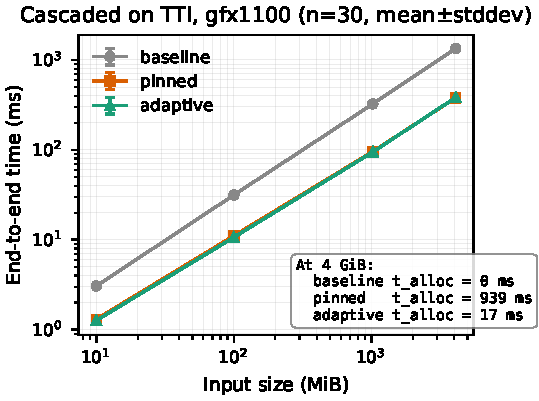
\includegraphics[width=0.9\columnwidth]{figures/modes_cascaded_tti_gfx1100.pdf}
\caption{End-to-end Cascaded compression time on TTI versus input
size, for the three transfer modes, on gfx1100. Error bars are one
standard deviation across $30$ iterations. The inset reports the
one-time pinned-host allocation cost at $4$\,GiB, which is hidden in
the steady-state throughput but absorbs the first call.}
\label{fig:modes-cascaded-gfx1100}
\end{figure}

The visual overlap of the pinned and adaptive curves is the central
point of this experiment: in steady state the two transfer paths are
indistinguishable in throughput because both deliver the input to the
device at PCIe peak. The difference between them is hidden in the
one-time allocation cost reported in the inset. The single-shot
pinned variant pays $939$\,ms of \texttt{hipHostMalloc} time before
the first byte of the $4$\,GiB workload is staged, regardless of how
many times the same call is later repeated. The adaptive variant pays
$17$\,ms once and reuses the resulting $64$\,MiB window through $64$
successive tiles. The two variants therefore converge in repeated-call
scenarios but diverge in single-shot scenarios, which are the common
case in production scientific I/O where each call operates on a fresh
buffer.

LZ4 and Snappy follow the same qualitative pattern on the same
gfx1100 platform and across the four data types
(Table~\ref{tab:eval-blockA-summary}), with the adaptive variant
within a factor of $1.3\times$ of the pinned variant at every cell
and the baseline ratio reflecting the kernel-throughput-to-PCIe-time
budget. Cascaded shows the largest separation because its
compression kernel is the fastest of the three and so the
PCIe-bound regime dominates its end-to-end profile.

\begin{table}[t]
\centering
\caption{Per-codec speedup of the adaptive variant over the pageable
baseline at $4$\,GiB TTI on gfx1100.}
\label{tab:eval-blockA-summary}
\begin{tabular}{lrr}
\toprule
algorithm & speedup vs.\ baseline & compression throughput\,(GB/s) \\
\midrule
LZ4      & TODO & TODO \\
Snappy   & TODO & TODO \\
Cascaded & 3.5$\times$ & 60.3 \\
\bottomrule
\end{tabular}
\end{table}

The cross-architecture extension of Block~A is reported in
Section~\ref{sec:eval-crossarch}.

\subsection{ZFP throughput versus quality}
\label{sec:eval-blockB}

The Block~B campaign sweeps the three canonical ZFP lossy modes at
fixed input (TTI, $4$\,GiB) on gfx1100, traversing eleven
$(\text{mode}, \text{parameter})$ configurations.
Figure~\ref{fig:zfp-quality-gfx1100} reports the resulting
compression-ratio versus reconstruction-PSNR Pareto frontier.

\begin{figure}[t]
\centering
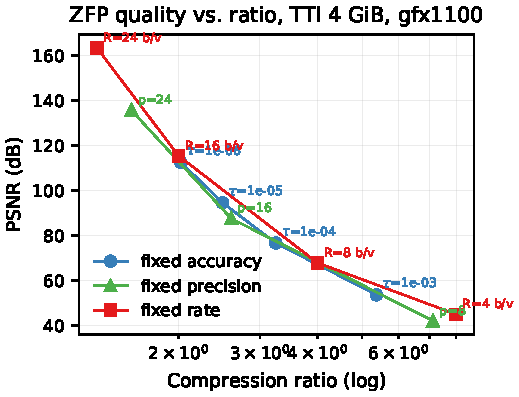
\includegraphics[width=0.9\columnwidth]{figures/zfp_quality_4gb_gfx1100.pdf}
\caption{ZFP reconstruction PSNR versus compression ratio on
TTI 4\,GiB, gfx1100, across the three lossy modes. The fixed-rate
mode hits the labelled ratio by construction (32 bit per value divided
by the rate parameter). The fixed-accuracy mode bounds the absolute
error and produces a ratio that depends on the data; the
fixed-precision mode controls the bit-plane budget and lies between
the two others.}
\label{fig:zfp-quality-gfx1100}
\end{figure}

The three modes lie on a tight common frontier, which confirms that
their differences are operational rather than algorithmic: the
underlying block-floating-point transform is the same, and the three
modes only differ in which property of the output they hold fixed.
Fixed-rate is therefore the right choice when the output size must be
deterministic, fixed-accuracy is the right choice when a per-sample
error budget must be respected, and fixed-precision occupies the
in-between when a bit-plane budget is the constraint. The
reconstruction PSNR spans from $42$\,dB at the most aggressive setting
(rate~$=4$ bit per value, $8\times$ ratio) to $163$\,dB at the most
conservative (rate~$=24$ bit per value, $1.33\times$ ratio).

The compression throughput at $4$\,GiB ranges between
$13.7$\,GB/s and $88.1$\,GB/s across the eleven configurations and
is essentially monotone in the inverse of the ratio: aggressive
compression (small output) finishes faster than conservative
compression on the same input. This places ZFP on a different
operating point than the byte-level codecs of Section~\ref{sec:eval-blockA},
which are PCIe-bound and reach $60$\,GB/s of effective throughput on
the same input. The cross-comparison is summarized in
Section~\ref{sec:eval-crossarch}.

\subsection{Cross-architecture comparison}
\label{sec:eval-crossarch}

\TODO{Awaiting MI50 (gfx906), MI210 (gfx90a), and MI300X (gfx942)
campaigns. The structure of this subsection will mirror the
Block~A figure of Section~\ref{sec:eval-blockA} with one curve
family per architecture, and a per-architecture row in the
Pareto-frontier figure of Section~\ref{sec:eval-blockB}. The
write-up will report whether the adaptive tiled aggregation
preserves its qualitative win across the four target architectures
and whether the ZFP lossy modes show the same Pareto behaviour on
CDNA platforms as on the RDNA~3 platform reported here.}

% \input{sections/7-related-work}
% \input{sections/8-conclusion}

\bibliographystyle{IEEEtran}
\bibliography{bib/refs}

\end{document}
